\documentclass{beamer}


\usecolortheme[named=teal]{structure}
\usepackage{amsmath,amssymb,enumerate}
\setbeamertemplate{navigation symbols}{}
\setbeamerfont{frametitle}{size = {\large}}


\usepackage{graphicx}
\usepackage{float}
\usepackage{caption}                 
\usepackage{tikz}
% \usepackage{mathpazo}
\usepackage{palatino}
% \usepackage{dejavu}

% \usepackage{pgfpages}              % uncomment these and compile 
% \pgfpagesuselayout{8 on 1}         % to make a handout

\DeclareMathOperator{\num}{f}
\DeclareMathOperator{\Av}{Av}
\newcommand{\C}{\mathcal{C}}
\newcommand{\Avns}{\Av_n ^* 123 }
\newcommand{\Avn}{\Av_n   123 }
 

%===========================================================%
\begin{document}


\begin{frame}
  \title{Expected Patterns in Permutation Classes}
  \author{Cheyne Homberger}
  \institute{AMS East Sectional Meeting \\
      Rochester Institute of Technology}
  \maketitle
\end{frame}


\begin{frame}{Introduction}
  \pause 

  \begin{block}{Example}
    The permutation $3 \ 1 \ 5 \ 2 \ 4$ contains the
    pattern $3 \ 1 \ 2$ twice (the first, second and forth entries and
    the third, forth and fifth).
  \end{block}
  \pause

  \begin{block}{Example}
    The set $\{ 2341 , 1234, 4321 \} $ contains the pattern $123$
    exactly $5$ times. 
  \end{block}
\end{frame}


\begin{frame}{Motivation}
  \begin{block}{Fact}
    In $S_n$, the number of occurrences of a specific pattern depends only on
    the length of the pattern. 
  \end{block}
  \pause
  \begin{block}{Question}
  How does this change when we replace $S_n$ with a 
  proper permutation class?
  \end{block}
  \pause

  \begin{figure}
  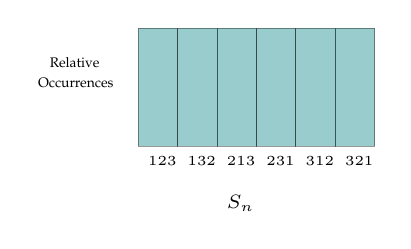
\begin{tikzpicture}
  [scale = .5]
  \foreach \x in {0,1,2,3,4,5}{
    \draw[color = black, fill = teal, opacity = .4] (\x,0) rectangle (\x+1, 3);
  }
  \draw (0, 0) node[anchor=north west] {\tiny $123$};
  \draw (1, 0) node[anchor=north west] {\tiny $132$};
  \draw (2, 0) node[anchor=north west] {\tiny $213$};
  \draw (3, 0) node[anchor=north west] {\tiny $231$};
  \draw (4, 0) node[anchor=north west] {\tiny $312$};
  \draw (5, 0) node[anchor=north west] {\tiny $321$};
  \draw (2,-1) node[anchor=north west] {\scriptsize $S_n$};
  \draw (-2.5, 2.5) node[anchor=north west] {\tiny Relative};
  \draw (-2.8, 2) node[anchor=north west] {\tiny Occurrences};
  \end{tikzpicture} \hspace{2pc} \pause
  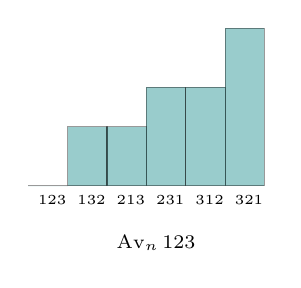
\begin{tikzpicture}
  [scale = .5]
  \foreach \x/\y in {0/0, 1/1.5, 2/1.5, 3/2.5, 4/2.5, 5/4}{
    \draw[color = black, fill = teal, opacity = .4] (\x,0) rectangle (\x+1,\y );
  }
  \draw (0, 0) node[anchor=north west] {\tiny $123$};
  \draw (1, 0) node[anchor=north west] {\tiny $132$};
  \draw (2, 0) node[anchor=north west] {\tiny $213$};
  \draw (3, 0) node[anchor=north west] {\tiny $231$};
  \draw (4, 0) node[anchor=north west] {\tiny $312$};
  \draw (5, 0) node[anchor=north west] {\tiny $321$};
  \draw (2,-1) node[anchor=north west] {\scriptsize $\Av_n 123$};
  \end{tikzpicture}
  \end{figure}
\end{frame}


\begin{frame}{Notation}
  \pause

  \begin{block}{Definition}
    For any permutations $q$ and $p$, denote by $\num_q (p)$ the
    number of occurrences of the pattern $q$ in the permutation $p$. 
  \end{block}
  \pause
  
  \begin{block}{Example}
    $$ \num_{21} (23154) = 3$$
  \end{block}

  \pause
  
  \begin{block}{Definition}
    Similarly, for a pattern $q$ and a set $S$ of permutations,
    define 
    $$ \num_q (S) = \sum_{p \in S} \num_q(p). $$
    \pause
    $$\num_{231}(S_n) = \frac{1}{n+1} \binom{2n}{n} = c_n$$
  \end{block}

\end{frame}


\begin{frame}{Previous Results}

  \begin{block}{Theorem (Cheng, Eu, Fu)}
    The total number of inversions in the set $\Av_n 321 $ is 
    $$  4^{n-1} - \binom{2n-1}{n}.$$
  \end{block}
    
  \pause 

  \begin{block}{Theorem (B\'ona)}
    In $\Av_n 132$, the pattern $123$ is the least common, $321$ is the most
    common, and $\num_{213} = \num_{231} = \num_{312}$. \\
    \pause
    In addition, let $q, t$ be any two non-empty patterns  which end in their
    largest entry, and let $i_u$ denote the increasing permutation of lenght
    $u$. Then
    {\Large
    $$ \num_{(q \ominus t ) \oplus i_u} = \num_{(q \oplus i_u) \ominus t}$$
    }
  \end{block}
    
\end{frame}




\begin{frame}{Data}
  \pause
  \vspace{-1pc}
  $$ \Av 132 $$
  $$\begin{array}{c|c|c|c|c|c|c}
      \text{length} & 123 & 132 & 213 & 231
      & 312 & 321 \\
      \hline
     3  & 1     &    0  &    1 &    1 &    1 &    1  \\
     4  & 10    &    0  &   11 &   11 &   11 &   13  \\
     5  & 68    &    0  &   81 &   81 &   81 &  109  \\
     6  & 392   &    0  &  500 &  500 &  500 &  748  \\ 
     7  & 2063  &    0  & 2794 & 2794 & 2794 & 4570   
   \end{array}
  $$
  \pause
  $$\Av 123 $$
  $$\begin{array}{c|c|c|c|c|c|c}
      \text{length} & 123 & 132 & 213 & 231
      & 312 & 321 \\
      \hline
      3  & 0     &    1  &    1 &    1 &    1 &    1  \\
      \pause
      4  & 0     &    9  &    9 &   11 &   11 &   16  \\
      \pause
      5  & 0     &    57 &   57 &   81 &   81 &  144  \\
      6  & 0     &   312 &  312 &  500 &  500 & 1016  \\ 
      7  & 0     &  1578 & 1578 & 2794 & 2794 & 6271   
    \end{array}
  $$
\end{frame}


\begin{frame}{Preliminaries}
  \pause

  \begin{block}{Theorem}
    % $$\num_{12}( \Av_n 123) = \sum_{k=1}^{n-1} c_k 4^{n-k-1} = 
    %   4^{n-1} - \binom{2n-1}{n}$$
    $$\sum_{n \geq 0} \num_{12}(\Av_n 123) x^n = 
      \frac{1 - 2x - \sqrt{1-4x}}{2(1-4x)}.$$
  \end{block}

  \pause

  \begin{block}{Fact}
    $$ (\num_{12} + \num_{21})(\Avn)  = \binom{n}{2} c_n .$$ 
  \end{block}
\end{frame}

\begin{frame}{Preliminaries}
  
  \begin{block}{Fact}
    $$ (2 \num_{132} + 2 \num_{231} +
      \num_{321})(\Avn) = \binom{n}{3} c_n.$$
  \end{block}

  \pause

  \begin{block}{Proposition}
    $$ (4 \num_{132} + 2 \num_{231})(\Avn) =
      (n-2) \num_{12}(\Avn). $$
  \end{block}
  \pause

  \begin{proof}
    Rewrite as 
    $$ (n-2)\num_{12} - \num_{132} - \num_{213} = 
      \num_{231} + \num_{312}+ \num_{132} + \num_{213}. $$
    Both sides count the number of length three patterns with at least
    one non-inversion.
  \end{proof}

\end{frame}


% \begin{frame}{Preliminaries}
% 
%   \begin{block}{Lemma}
%     Let $a_n = \num_{132}(\Avn)$, $b_n = \num_{231}(\Avn)$, $d_n =
%     \num_{321}(\Avn)$, and $j_n = \num_{12}(\Avn)$. Let $A(x), B(x),
%     D(x), J(x)$ be their respective generating functions. Then 
%     $$ \begin{array}{ccccc}
%       2A(x) & + 2B(x) & + D(x) & = & \frac{x^3}{6} (C(x))''' \\
%       4A(x) & + 2B(x) & & =&  x^3(J(x)/x^2)' 
%       \end{array} $$
%   \end{block}
% 
% \end{frame}
  

\begin{frame}{Indecomposable Permutations}
\pause
  
  \begin{block}{Definition}
    We say that a permutation $p = p_1 p_2 \ldots p_n$ is
    \emph{decomposable} if there exists an integer $k$ so that each
    of the entries $p_1, \ldots p_k$ is greater than each of the
    entries $p_{k+1}, \ldots p_n$. Otherwise, we say that $p$ is
    \emph{indecomposable}
  \end{block}

  \pause

  \begin{block}{Example}
    The permutation $3 5 6 4 1 2$ is decomposable, as the entries
    $3564$ are larger than the entries $12$
  \end{block}

  \pause

  \begin{block}{Definition}
    Denote by $\Avns$ the set of indecomposable $n$-permutations which
    avoid $123$.
  \end{block}

\end{frame}


\begin{frame}{Indecomposable Permutations}

  \begin{block}{Fact}
    $|\Avns| = c_{n-1}$.
  \end{block}
  \pause

  \begin{proof}
    \vspace{.5pc}

    \begin{tikzpicture}[scale = .5]
      
      \draw[thick] (0,8) -- (0,0) -- (8,0) -- (8,8) -- (0,8);
      \node at (4,4) {$\Avn$};
      \node at (9,4) {$ = $};

      \draw (10,8) -- (10,6) -- (12,6) -- (12,8) -- (10,8);
      \node at (11,7) {\scriptsize $ \Avns$};

      \draw (12,6) -- (12,4) -- (14,4) -- (14,6) -- (12,6);
      \node at (13,5) {\scriptsize $ \Avns$};
      
      \node at (15,3) {$\ddots$};

      \draw (16,2) -- (16,0) -- (18,0) -- (18,2) -- (16,2);
      \node at (17,1) {\scriptsize $ \Avns$};
    \end{tikzpicture}

    \pause
    $$ C(x) = 1 + C^*(x) + C^*(x)^2 + \ldots = \frac{1}{1 - C^*(x)}$$

    \vspace{-1pc}
    \pause
    $$ C^*(x) = \frac{C(x) - 1}{C(x)} =  xC(x).$$


  \end{proof}

\end{frame}


\begin{frame}{Indecomposable Permutations}

  \begin{block}{Fact}
    $|\Avns| = c_{n-1}$.
  \end{block}

  \begin{proof}[Alternate Proof]
    \vspace{.5pc}

    \begin{tikzpicture}[scale = .5]
      
      \draw[thick] (0,8) -- (0,0) -- (8,0) -- (8,8) -- (0,8);
      \node at (4,4) {$\Avn$};
      \node at (9,4) {$ = $};

      \draw (10,8) -- (10,6) -- (12,6) -- (12,8) -- (10,8);
      \node at (11,7) {\scriptsize $ \Avns$};

      \draw (12,6) -- (12,0) -- (18,0) -- (18,6) -- (12,6);
      \node at (15,3) {$ \Avn$};
    \end{tikzpicture}

    $$ C(x) = C^*(x) C(x) + 1$$
    
    \vspace{-1pc}
    $$ C^*(x) = \frac{C(x) - 1}{C(x)} =  xC(x).$$


  \end{proof}

\end{frame}


% \begin{frame}
%   \begin{block}{Lemma}
%     Let $a_n = \num_{132}(\Avn)$, $b_n = \num_{231}(\Avn)$, $d_n =
%     \num_{321}(\Avn)$, and $j_n = \num_{12}(\Avn)$. Let $A(x), B(x),
%     D(x), J(x)$ be their respective generating functions. Let $*$
%     denote the corresponding numbers for indecomposable permutations.
%     Then 
%     $$ \begin{array}{ccccc}
%       2A(x) & + 2B(x) & + D(x) & = & \frac{x^3}{6} (C(x))''' \\
%       4A(x) & + 2B(x) & & =&  x^3(J(x)/x^2)' \\
%       \pause
%       2A^*(x) & + 2B^*(x) & + D^*(x) & = & \frac{x^3}{6} (xC(x))'''\\
%       4A^*(x)& + 2B^*(x)& & =& x^3(J^*(x) /x^2)' 
%       \end{array} $$
%   \end{block}
% 
% \end{frame}


\begin{frame}{Solving the System}
  \begin{block}{\only<-2>{Conjectures}\uncover<3>{Corollary}}
    \pause
    $$ C(x) A(x)  = xJ(x) C'(x)$$
    % $$ C(x) A^*(x) = xF^*(x) C'(x) $$
    $$ A^*(x) + B^*(x) = \sum_{n\geq 0} \num_{213} \big(\Av_n^* 132
    \big) x^n $$ 
    $$ B^*(x) C(x) = 2xB(x) $$
    $$ A(x)+B(x) = 2\sum_{n\geq 0} \Big(\num_{213} \big( \Av ^*_n
    132 \big) + \num_{231} \big( \Av ^*_n 132 \big)\Big) x^n $$
    $$ A(x) + B(x) = xB^*(x) $$
    $$ J^*(x)  = 2A^*(x) $$
  \end{block}
\end{frame}


\begin{frame}

  \begin{block}{Lemma}
    $$A^*(x) = \frac{x^3C(x)}{(1-4x)^{3/2}}$$
  \end{block}

\end{frame}


\begin{frame}{One Last Definition}
  \pause
  
  \begin{block}{Definition}
    A \emph{Dyck path} of length $2n$ (or of semilength $n$) is a
    path in the plane from $(0,0)$ to $(2n,0)$ using steps $(1,1)$ and
    $(1,-1)$ which never crosses below the $x$-axis. 
  \end{block}
  \pause 

  \begin{block}{Example}
    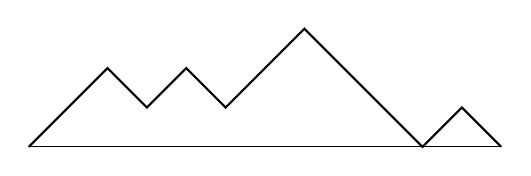
\begin{tikzpicture}[scale = .5, auto = center]
      \draw[thick] (0,2) -- (2,4) -- (3,3) -- (4,4) --
                   (5,3) -- (7,5) -- (10,2) -- (11,3) --
                   (12,2);
      \draw (0,2) -- (12,2);
      \end{tikzpicture}
      $ = UUDUDUUDDDUD.$
  \end{block}
  \pause

  \begin{block}{Fact}
    There are exactly $c_n$ Dyck paths of semilength $n$.   
  \end{block}

\end{frame}



\begin{frame}{Sketch of proof}

  \only<-12>{
    Let $p = 4 \ 3 \ 7 \ 6 \ 1 \ 5 \ 2 $, and count $213$ patterns. \\
    \hfill 
  }
  \only<13->{ Let $h_{n,k}$ denote the total number of peaks at height
  $k$ in all Dyck paths of semilength $n$. 
  Let $H(x,u) = \sum_{n,k \geq 0} h_{n,k} x^n u^k$. \\
  \vspace{-.4pc} }

  \begin{figure}[center]
  
  % lots of pictures... not the prettiest code
    \only<1>{
      \begin{tikzpicture}[scale = .7, auto = center]
        \draw[thick, color =  white] (0,8) -- (0,0) -- (8,0);
      \end{tikzpicture}
      }

    \only<2>{
      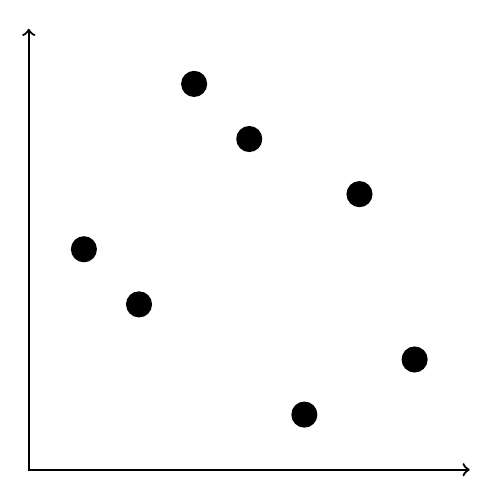
\begin{tikzpicture}[scale = .7, auto = center]
        \draw[thick, <->] (0,8) -- (0,0) -- (8,0);
        \node[circle, fill=black] at (1,4) {};
        \node[circle, fill=black] at (2,3) {};
        \node[circle, fill=black] at (3,7) {};
        \node[circle, fill=black] at (4,6) {};
        \node[circle, fill=black] at (5,1) {};
        \node[circle, fill=black] at (6,5) {};
        \node[circle, fill=black] at (7,2) {};
      \end{tikzpicture}
    }

    \only<3>{ 
      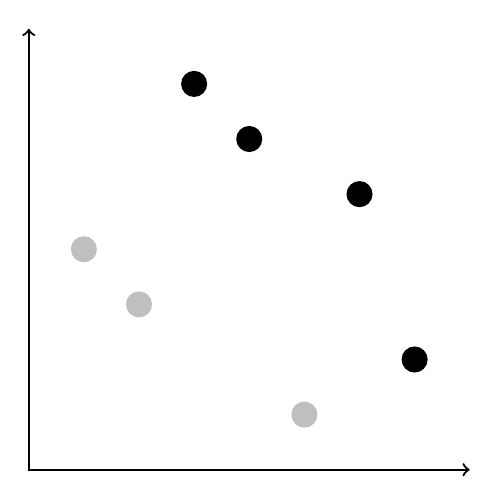
\begin{tikzpicture}[scale = .7, auto = center]
        \draw[thick, <->] (0,8) -- (0,0) -- (8,0);
        \node[circle, fill=lightgray] at (1,4) {};
        \node[circle, fill=lightgray] at (2,3) {};
        \node[circle, fill=black] at (3,7) {};
        \node[circle, fill=black] at (4,6) {};
        \node[circle, fill=lightgray] at (5,1) {};
        \node[circle, fill=black] at (6,5) {};
        \node[circle, fill=black] at (7,2) {};
      \end{tikzpicture}
    }

    \only<4>{ 
      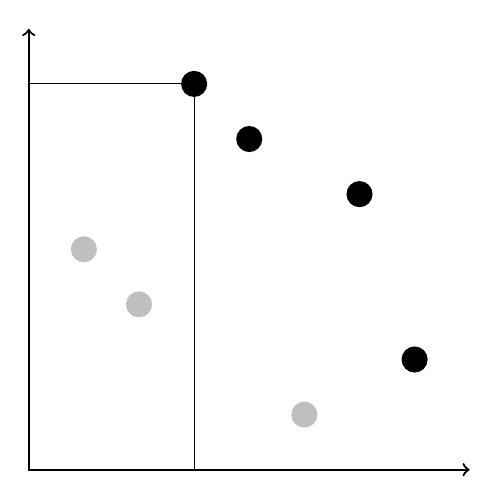
\begin{tikzpicture}[scale = .7, auto = center]
        \draw[thick, <->] (0,8) -- (0,0) -- (8,0);
        \node[circle, fill=lightgray] at (1,4) {};
        \node[circle, fill=lightgray] at (2,3) {};
        \node[circle, fill=black] at (3,7) {};
        \node[circle, fill=black] at (4,6) {};
        \node[circle, fill=lightgray] at (5,1) {};
        \node[circle, fill=black] at (6,5) {};
        \node[circle, fill=black] at (7,2) {};
        \draw (0,7) -- (3,7) -- (3,0);
      \end{tikzpicture}
    }

    \only<5>{ 
      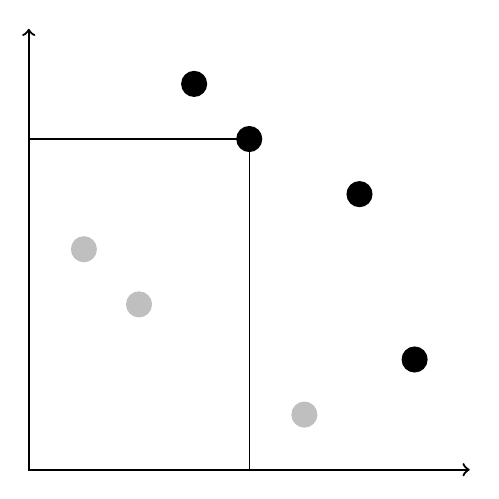
\begin{tikzpicture}[scale = .7, auto = center]
        \draw[thick, <->] (0,8) -- (0,0) -- (8,0);
        \node[circle, fill=lightgray] at (1,4) {};
        \node[circle, fill=lightgray] at (2,3) {};
        \node[circle, fill=black] at (3,7) {};
        \node[circle, fill=black] at (4,6) {};
        \node[circle, fill=lightgray] at (5,1) {};
        \node[circle, fill=black] at (6,5) {};
        \node[circle, fill=black] at (7,2) {};
        \draw (0,6) -- (4,6) -- (4,0);
      \end{tikzpicture}
    }

    \only<6>{ 
      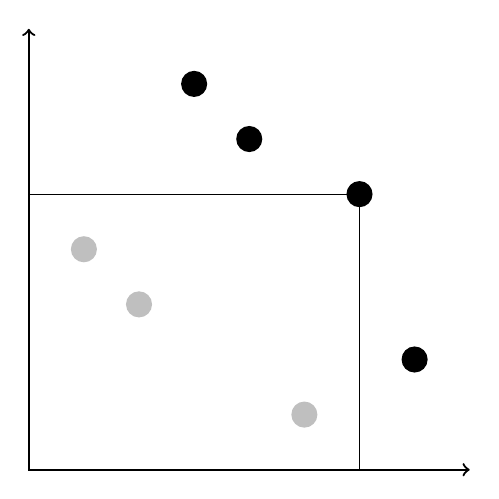
\begin{tikzpicture}[scale = .7, auto = center]
        \draw[thick, <->] (0,8) -- (0,0) -- (8,0);
        \node[circle, fill=lightgray] at (1,4) {};
        \node[circle, fill=lightgray] at (2,3) {};
        \node[circle, fill=black] at (3,7) {};
        \node[circle, fill=black] at (4,6) {};
        \node[circle, fill=lightgray] at (5,1) {};
        \node[circle, fill=black] at (6,5) {};
        \node[circle, fill=black] at (7,2) {};
        \draw (0,5) -- (6,5) -- (6,0);
      \end{tikzpicture}
    }

    \only<7>{ 
      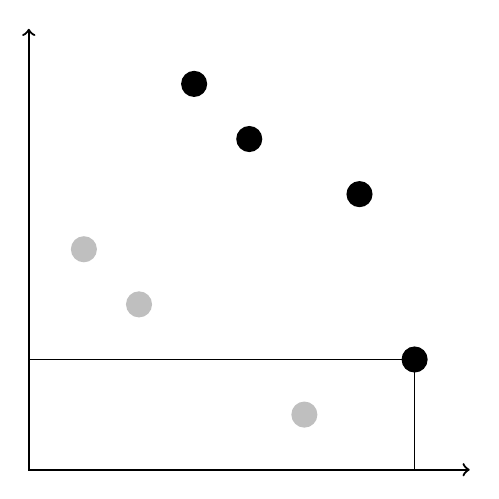
\begin{tikzpicture}[scale = .7, auto = center]
        \draw[thick, <->] (0,8) -- (0,0) -- (8,0);
        \node[circle, fill=lightgray] at (1,4) {};
        \node[circle, fill=lightgray] at (2,3) {};
        \node[circle, fill=black] at (3,7) {};
        \node[circle, fill=black] at (4,6) {};
        \node[circle, fill=lightgray] at (5,1) {};
        \node[circle, fill=black] at (6,5) {};
        \node[circle, fill=black] at (7,2) {};
        \draw (0,2) -- (7,2) -- (7,0);
      \end{tikzpicture}
    }

    \only<8>{ 
      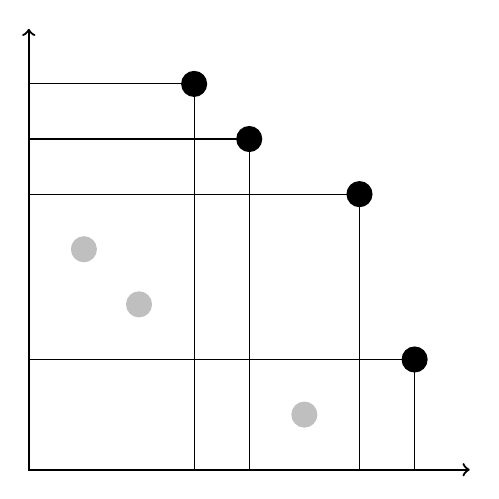
\begin{tikzpicture}[scale = .7, auto = center]
        \draw[thick, <->] (0,8) -- (0,0) -- (8,0);
        \node[circle, fill=lightgray] at (1,4) {};
        \node[circle, fill=lightgray] at (2,3) {};
        \node[circle, fill=black] at (3,7) {};
        \node[circle, fill=black] at (4,6) {};
        \node[circle, fill=lightgray] at (5,1) {};
        \node[circle, fill=black] at (6,5) {};
        \node[circle, fill=black] at (7,2) {};
        \draw (0,7) -- (3,7) -- (3,0);
        \draw (0,6) -- (4,6) -- (4,0);
        \draw (0,5) -- (6,5) -- (6,0);
        \draw (0,2) -- (7,2) -- (7,0);
      \end{tikzpicture}
    }

    \only<9>{ 
      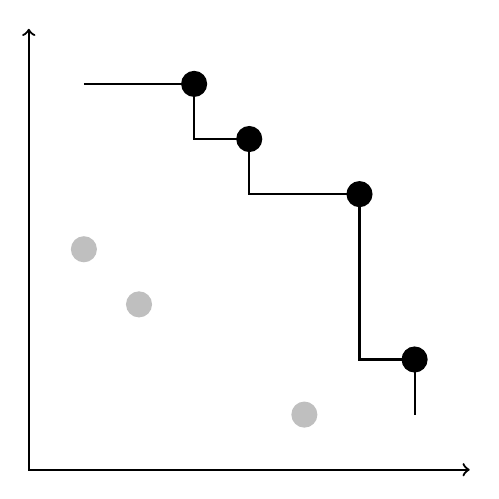
\begin{tikzpicture}[scale = .7, auto = center]
        \draw[thick, <->] (0,8) -- (0,0) -- (8,0);
        \node[circle, fill=lightgray] at (1,4) {};
        \node[circle, fill=lightgray] at (2,3) {};
        \node[circle, fill=black] at (3,7) {};
        \node[circle, fill=black] at (4,6) {};
        \node[circle, fill=lightgray] at (5,1) {};
        \node[circle, fill=black] at (6,5) {};
        \node[circle, fill=black] at (7,2) {};
        \draw[thick] (1,7) -- (3,7) -- (3,6) -- (4,6) --
                     (4,5) -- (6,5) -- (6,2) -- (7,2) --
                     (7,1);
      \end{tikzpicture}
    }

    \only<10>{ 
      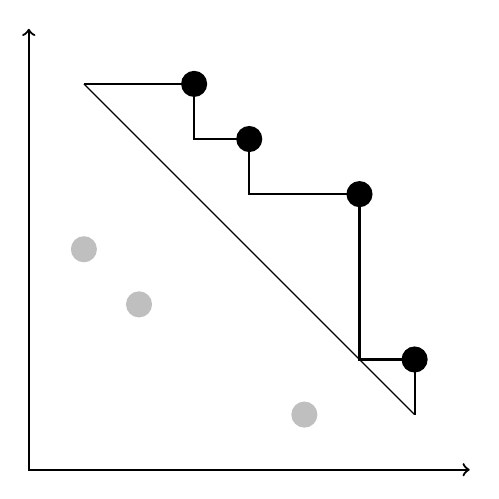
\begin{tikzpicture}[scale = .7, auto = center]
        \draw[thick, <->] (0,8) -- (0,0) -- (8,0);
        \node[circle, fill=lightgray] at (1,4) {};
        \node[circle, fill=lightgray] at (2,3) {};
        \node[circle, fill=black] at (3,7) {};
        \node[circle, fill=black] at (4,6) {};
        \node[circle, fill=lightgray] at (5,1) {};
        \node[circle, fill=black] at (6,5) {};
        \node[circle, fill=black] at (7,2) {};
        \draw[thick] (1,7) -- (3,7) -- (3,6) -- (4,6) --
                     (4,5) -- (6,5) -- (6,2) -- (7,2) --
                     (7,1);
        \draw (1,7) -- (7,1);
      \end{tikzpicture}
    }

    \only<11>{
      \begin{tikzpicture}[scale = .7, auto = center]
        \draw[thick, color =  white] (0,8) -- (0,0) -- (8,0);
        \draw[thick] (0,2) -- (2,4) -- (3,3) -- (4,4) --
                     (5,3) -- (7,5) -- (10,2) -- (11,3) --
                     (12,2);
        \draw (0,2) -- (12,2);
      \end{tikzpicture}
    }

    \only<12,13>{
      \begin{tikzpicture}[scale = .7, auto = center]
        \draw[thick, color =  white] (0,8) -- (0,0) -- (8,0);
        \draw[thick] (0,2) -- (2,4) -- (3,3) -- (4,4) --
                     (5,3) -- (7,5) -- (10,2) -- (11,3) --
                     (12,2);
        \draw (0,2) -- (12,2);
        
        \node at (2,5) {2};
        \node at (4,5) {2};
        \node at (7,6) {3};
        \node at (11,4) {1};
      \end{tikzpicture}
    }

    \only<14>{
      \begin{tikzpicture}[scale = .7, auto = center]
        \draw[thick, color =  white] (0,8) -- (0,0) -- (8,0);
        \draw[thick] (0,2) -- (2,4) -- (3,3) -- (4,4) --
                     (5,3) -- (7,5) -- (10,2) -- (11,3) --
                     (12,2);
        \draw (0,2) -- (12,2);
        \draw (1,3) -- (9,3);
        \draw (10,1) -- (10,5);
      \end{tikzpicture}
    }

    \only<15>{
      \vspace{.1pc}

      \begin{tikzpicture}[scale = .7, auto = center]
        \draw[thick, color =  white] (0,8) -- (0,0) -- (8,0);
        \draw[thick] (0,2) -- (2,4) -- (3,3) -- (4,4) --
                     (5,3) -- (7,5) -- (10,2) -- (11,3) --
                     (12,2);
        \draw (0,2) -- (12,2);
        \draw (1,3) -- (9,3);
        \draw (10,1) -- (10,5);

        \node at (5,5) {$uH(x,u)$};
        \node at (11,5) {$H(x,u)$};
      \end{tikzpicture}
    }

  \end{figure}


    $$ \only<4-13>{\num_{213}(p)}  \uncover<4-13>{ = \binom{2}{2}}
    \only<5-13>{ + \binom{2}{2}} \only<6-13>{ + \binom{3}{2}}
    \only<7-13>{ + \binom{1}{2}} \only<8-13>{ = 5  }
    \only<14->{H(x,u) = } 
    \only<15->{ux (H(x,u) + 1) C(x) + xC(x) H(x,u)}  
    $$ 

\end{frame}


\begin{frame}{Sketch of proof} 
  
  Let $h_{n,k}$ denote the total number of peaks at height
  $k$ in all Dyck paths of semilength $n$. 
  Let $H(x,u) = \sum_{n,k \geq 0} h_{n,k} x^n u^k$. 
  
  \vspace{2pc}

  $$H(x,u) = \frac{uxC(x)}{1-uxC(x)-xC(x)}.$$
  \pause
  $$ A^*(x) = \sum_{n \geq 0} \binom{k}{2} h_{n-1,k} x^n$$
  \pause
  $$ \begin{aligned}
    A^*(x) &= \frac{\left. x \partial_u ^2 H(x)\right|_{u=1}}{2} \\
         \pause
         &= \frac{x^3C(x)}{(1-4x)^{3/2}} \\ 
         \pause
         &= x^3 + 7x^4 + 38x^5 + 187^6 + \ldots
      \end{aligned} $$
    \pause
    \begin{flushright} $ \qed $ \end{flushright}

\end{frame}


\begin{frame}{Corollaries}
  \pause
  \begin{block}{Corollary}
    $$ \num_{231}(\Avn) = \num_{231}(\Av_n 132)$$
  \end{block}
\end{frame}


\begin{frame}{Corollaries}

    $$ A(x) = \frac{x-1}{2(1-4x)} - \frac{3x-1}{2(1-4x)^{3/2}}$$

    $$B(x) = \frac{3x-1}{(1-4x)^{2}} - \frac{4x^2 - 5x +
    1}{(1-4x)^{5/2}}$$

    $$ D(x) =   \frac{ 8x^3 - 20x^2 + 8x - 1}{(1-4x)^{2}} 
      - \frac{36x^3 - 34x^2 + 10x - 1}{(1-4x)^{5/2}} $$ 

\end{frame}




\begin{frame}{Corollaries}

  $$ a_n = \frac{n+2}{4} \binom{2n}{n} - 3 \cdot 2^{2n-3} $$\\[.5pc]
  $$ b_n = (2n-1) \binom{2n-3}{n-2} - (2n+1)\binom{2n-1}{n-1} + 
     (n+4) \cdot 2^{2n-3}$$\\[.5pc]
  $$ \begin{aligned} d_n 
      &= \frac{1}{6} \binom{2n+5}{n+1} \binom{n+4}{2} 
      - \frac{5}{3} \binom{2n+3}{n} \binom{n+3}{2} \\
      &+ \frac{17}{3} \binom{2n+1}{n-1} \binom{n+2}{2} 
      - 6\binom{2n-1}{n-2} \binom{n+1}{2} - (n+1) \cdot 4^{n-1}.
    \end{aligned}
  .$$

\end{frame}


\begin{frame}{Corollaries}

  $$ a_n \sim \sqrt{\frac{n}{\pi}} 4^n$$
  $$ b_n \sim \frac{n}{2} 4^n $$
  $$ d_n \sim \frac{8}{3} \sqrt{\frac{n^3}{\pi}} 4^n. $$

\end{frame}


\begin{frame}{Larger patterns}
  \pause
  \begin{block}{Lemma}
    $$ \begin{array}{ccccc}
      2A(x) & + 2B(x) & + D(x) & = & \frac{x^3}{6} (C(x))'''\\
      4A(x) & + 2B(x) & & =&  x^3(J(x)/x^2)' 
      \end{array} $$
  \end{block}
  \pause
  \begin{block}{Theorem}
    For large enough $n$, the descending pattern of length $k$ occurs
    more often than any other length $k$ pattern in $\Avn$. 
  \end{block}
\end{frame}

\begin{frame}{Further Directions}
  \pause

  \begin{block}{Note}
    No other 'surprising' symmetries found for patterns of length $5$ in $\Av
    123$, or for any patterns in $\Av q$, for $|q| = 4$. 
  \end{block}
  \pause
  \begin{block}{Note}
    The increasing and decreasing patterns are not always the extremes of the
    class: $\num_{123} (\Av 2413) = \num_{321} (\Av 2413) $ 
  \end{block}
  \pause

  \vspace{1pc}

  \begin{center}
  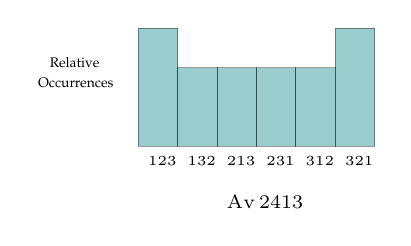
\begin{tikzpicture}
  [scale = .5]
  \foreach \x/\y in {0/3,1/2,2/2,3/2,4/2,5/3}{
    \draw[color = black, fill = teal, opacity = .4] (\x,0) rectangle (\x+1,\y);
  }
  \draw (0, 0) node[anchor=north west] {\tiny $123$};
  \draw (1, 0) node[anchor=north west] {\tiny $132$};
  \draw (2, 0) node[anchor=north west] {\tiny $213$};
  \draw (3, 0) node[anchor=north west] {\tiny $231$};
  \draw (4, 0) node[anchor=north west] {\tiny $312$};
  \draw (5, 0) node[anchor=north west] {\tiny $321$};
  \draw (2,-1) node[anchor=north west] {\scriptsize $\Av 2413$};
  \draw (-2.5, 2.5) node[anchor=north west] {\tiny Relative};
  \draw (-2.8, 2) node[anchor=north west] {\tiny Occurrences};
  \end{tikzpicture} 
  \end{center}


\end{frame}


% \begin{frame}
%   \begin{block}{\hspace{6pc}\Large Thanks for listening!}
%   \end{block}
% \end{frame}

\end{document}
